\vspace*{-1em}
\section{Introduction}
% \Glspl{CNN} for image classification learn faster and generalize better than non-convolutional ones, because convolutions reduce the number of learned parameters and inject a strong and generally correct inductive bias: 
% if a local feature is useful in one image location, the same feature is likely to be useful in other locations.
% It is tempting to embed even stronger inductive biases by replicating features across scale, orientation and other affine degrees of freedom, but this quickly leads to cumbersome high-dimensional feature maps \citep{Cohen2016steerable}.
% 
\Gls{CNN} work better than networks without weight-sharing because of their inductive bias: if a local feature is useful in one image location, the same feature is likely to be useful in other locations. It is tempting to exploit other effects of viewpoint changes by replicating features across scale, orientation and other affine degrees of freedom, but this quickly leads to cumbersome high-dimensional feature maps. %%\citep{Cohen2016steerable}.
%% its a bit mean to blame taco and max for this and we refer to them later anyway.

An alternative to replicating features across the non-translational degrees of freedom is to explicitly learn transformations between the natural coordinate frame of a whole object and the natural coordinate frames of each of its parts.   Computer graphics relies on such object$\rightarrow$part coordinate transformations to represent the geometry of an object in a viewpoint-invariant manner. Moreover, there is strong evidence that, unlike standard \gls{CNN}s, human vision also relies on coordinate frames: imposing an unfamiliar coordinate frame on a familiar object makes it difficult to recognize the object or its geometry \citep{Rock73, Hinton79}.

A neural system can learn to reason about transformation between objects, their parts and the viewer, but each of the transformations is likely to require different representation.
An \gls{OP} is viewpoint-invariant and is naturally coded by learned weights.  
The relationship of an object or part to the viewer changes with the viewpoint (it is viewpoint-equivariant) and is naturally coded using neural activations\footnote{
    This may explain why accessing perceptual knowledge about objects, when they are not visible, requires creating a mental image of the object with a specific viewpoint.
}.
With this representation, pose of a single object is represented by its relationship to the viewer.
Consequently, representing a single object does not necessitate replicating neural activations across space, unlike in \glspl{CNN}.
It is only processing two (or more) different instances of the same type of object in parallel that requires spatial replicas of both model parameters and neural activations.
% So the stride of the replication of object and part capsules can be determined by the sparsity of that type of object or part in the image and can typically be much larger for more complex objects because they are sparser. 

In this paper we propose the \gls{SCAu}, which has two stages (\cref{fig:capsule_arch}). The first stage, the \gls{PCAu}, segments an image into constituent parts, infers their poses, and reconstructs each image pixel as a mixture of the pixels of transformed part templates.
The second stage, the \gls{OCAu}, tries to organize discovered parts and their poses into a smaller set of objects that can explain the part poses using a separate mixture of predictions for each part. 
Every object capsule contributes components to each of these mixtures by multiplying its pose---the \gls{OV}---by the relevant \glsreset{OP}\gls{OP}\footnote{The type of a part capsule may determine which, if any, of an object's parts contribute to the mixture used to model the pose of an already discovered part}.

Stacked Capsule Autoencoders (\Cref{sec:caps_decoders}) capture spatial relationships between whole objects and their parts when trained on unlabelled data.
The vectors of presence probabilities for the object capsules tend to form tight clusters, and when we assign a class to each cluster we achieve state-of-the-art results for unsupervised classification on \textsc{svhn} (55\%) and near state-of-the-art on \textsc{mnist} (98.5\%), which can be further improved to 67\% and 99\%, respectively, by learning fewer than 300 parameters. We also present promising proof-of-concept results on \textsc{cifar10} (\Cref{sec:experiments}).
%
We describe related work in \Cref{sec:related_work} and discuss implications of our work and future  directions in \Cref{sec:discussion}.

\begin{figure}
    \centering
    \begin{minipage}[c]{0.68\linewidth}
        \centering
        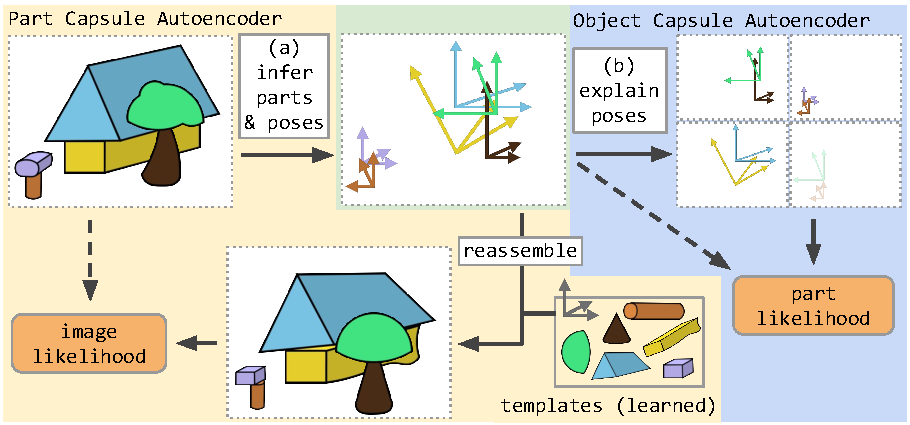
\includegraphics[width=\linewidth]{figs/blocks_v4}
        % \vspace*{-1.5em}
    \end{minipage}
    \hfill
    \begin{minipage}[c]{0.3\linewidth}
        \centering
        \caption{
            Stacked Capsule Autoencoder (\textsc{scae}):
            % \arcfull{}{SCA}
            (a) \textit{part} capsules segment the input into parts and their poses. The poses are then used to reconstruct the input by affine-transforming learned templates.
            (b) \textit{object} capsules try to arrange inferred poses into objects, thereby discovering underlying structure.
            \textsc{scae} is trained by maximizing image and part log-likelihoods subject to sparsity constraints.
        }
        \label{fig:capsule_arch}
        % \vspace*{-1.5em}
    \end{minipage}
    \vspace*{-.75em}
\end{figure}

% \Gls{SCA} has two stages (\cref{fig:capsule_arch}).
% Its first (\!\ie bottom) stage, \gls{ICAE}, segments an image into constituent parts, infers their poses, and reconstructs the image as a mixture of transformed parts.
% The second (top) stage, \gls{CAE}, tries to organize discovered parts and their poses into objects, where part poses \apart{} are derived from mixtures of predictions made by objects \awhole{}.
% Since each part is explained by a separate mixture, we do not need to route predictions between mixtures.
% This justifies dispensing with iterative procedures during inference, which can now be amortized using an arbitrary feed-forward encoder.
% The encoder's ability to deal with different viewpoints is not built-in; instead it is learned by doing inference for the affine-aware decoder.
% As \gls{SCA} is unsupervised, it can leverage potentially unlimited amounts of unlabelled data.
% % \yw{maybe say that the model is an autoencoder, where the decoder is structured with the assumptions about the geometries of objects as before? also maybe give some intuition about the decoder structuring the encoder to learn the structure we want it to learn (not sure if that makes sense)?}

